\documentclass[a4paper,12pt]{article}

\usepackage{fourier}
\usepackage[T1]{fontenc}


\usepackage{lscape}
\usepackage{amsmath}
%\usepackage{framed,enumerate}
%\usepackage{cite}
%\usepackage{color}
\usepackage[usenames,dvipsnames,svgnames,table]{xcolor}
\usepackage[justification=centering]{caption}
\usepackage{ragged2e,float}
\usepackage{subcaption,chngcntr}
%\usepackage[numbered]{mcode}
\usepackage{pgfplots}
\usepackage{tocloft,lipsum}
\usepackage{geometry,graphicx}
\usepackage{tabularx}
\usepackage{multirow}
\usepackage{tabstackengine}
\setstackEOL{@}
\setstackTAB{*}
\geometry{left=20mm,right=20mm,top=20mm,bottom=20mm}
\usepackage{gantt}
\usepackage{tikz}
\usetikzlibrary{shapes,arrows}

% FOR TIKZ AND LABELS
\newlength\figureheight
\newlength\figurewidth
\counterwithin{figure}{section}
\counterwithin{equation}{section}
\counterwithin{table}{section}
%\counterwithin{figure}{subsection}
%\counterwithin{figure}{subsubsect--ion}

% ROBOTO TITLES
\usepackage{titlesec}
\newcommand\roboto[1]{{\usefont{T1}{custom}{m}{n} #1 }}
%\titleformat*{\section}{\Large\roboto}
%\titleformat*{\subsection}{\large\roboto}
%\titleformat*{\subsubsection}{\roboto}
%\renewcommand{\cfttoctitlefont}{\Large\roboto} % contents title
%\renewcommand{\cftloftitlefont}{\Large\roboto} % list of figures title
%\renewcommand{\cftlottitlefont}{\Large\roboto} % list of tables title
\renewcommand{\cftsecleader}{\cftdotfill{\cftdotsep}} % toc dots

% SUBSUBSUBSECTION
\titleclass{\subsubsubsection}{straight}[\subsection]
\newcounter{subsubsubsection}[subsubsection]
\renewcommand\thesubsubsubsection{\thesubsubsection.\arabic{subsubsubsection}}
\titleformat{\subsubsubsection} 
{\normalfont\normalsize\bfseries}{\thesubsubsubsection}{1em}{}
\titlespacing*{\subsubsubsection}
{0pt}{3.25ex plus 1ex minus .2ex}{1.5ex plus .2ex}
\makeatletter
\def\toclevel@subsubsubsection{4}
\def\l@subsubsubsection{\@dottedtocline{4}{7em}{4em}}
\makeatother
\setcounter{secnumdepth}{4}
\setcounter{tocdepth}{4}

\usepackage{fancyhdr}
\pagestyle{fancy}
\fancyhf{}
\renewcommand{\headrulewidth}{0pt}
\rfoot{\thepage}
\lfoot{\textcolor{gray}{SnapSat PDR Summary Issue 1}} 

\usepackage{setspace}
%\singlespacing
%\onehalfspacing
%\doublespacing
\setstretch{1.1}

%TABLES
\usepackage{array}
\newcolumntype{L}[1]{>{\raggedright\let\newline\\\arraybackslash\hspace{0pt}}m{#1}}
\newcolumntype{C}[1]{>{\centering\let\newline\\\arraybackslash\hspace{0pt}}m{#1}}
\newcolumntype{R}[1]{>{\raggedleft\let\newline\\\arraybackslash\hspace{0pt}}m{#1}}


% SHORTCUTS
\renewcommand{\deg}{\ensuremath{^\circ}}
%\newcommand{\F}[1]{\ensuremath{F_{#1}}}
%\newcommand{\M}[1]{\ensuremath{M_{#1}}}
\newcommand{\tf}[2]{G_{\delta_#1}^{#2}(s)}
\newcommand{\bmat}[2]{\setstackgap{L}{1.2\baselineskip} \fixTABwidth{T} \setstacktabbedgap{#1} \bracketMatrixstack{#2}}
\newcommand{\vertmat}[2]{\setstackgap{L}{1.2\baselineskip} \fixTABwidth{T} \setstacktabbedgap{#1} \vertMatrixstack{#2}}
\newcommand{\tikzpic}[4]{\centering 
    \setlength\figurewidth{#1\linewidth} \setlength\figureheight{#2\linewidth} \input{#3} \caption{#4}}
\newcommand{\pic}[3]{\centering 
    \includegraphics[width=#1\linewidth]{#2} \caption{#3}}
%\newcommand{\unit}[2]{\frac{\text{#1}}{\text{#2}}}

\begin{document}
    
%%\begin{titlepage}

\thispagestyle{empty}
\begin{center}
\begin{minipage}{\linewidth}
    \centering
%University logo
    
\includegraphics[width=6.5cm]{logo.png}
    \par
    \vspace{1.2cm}
    {\textsc{School of Aerospace Mechanical and Mechatronic Engineering \\ \vspace{0.3cm}
            AERO3760: Space Engineering 2}}
   \vspace{0.7cm}
%Thesis title
	\hrule
    \vspace{1cm}
    {{\LARGE\bf{ Group E: SnapSat\\\vspace{0.4cm}Data Package Document 1 \\Critical Design Review }\par}}

    \vspace{1cm}
    \hrule
    \vspace{1.3cm}
     {\large \textsc{21 August 2015}}
\vspace{1.3cm}
%Author's name
    \begin{table}[H]
        \centering
        %\caption{Team Member Details and Contributions}
        \vspace{0.2cm}
        \label{tab:maxturbulencealpha}
        {\renewcommand{\arraystretch}{1.7}%
            \begin{tabular}{|>{\centering\arraybackslash}m{6cm}|>{\centering\arraybackslash}m{9cm}|}
                \hline
                \textbf{Name and Email} & \textbf{Role and Responsibility} \\ \hline\hline
                James Allworth | 312073038  jall8741@uni.sydney.edu.au & \textit{Attitude Determination and Control System} \newline TASKS  \\\hline
                Thomas Forbutt | 312101058  tfor8012@uni.sydney.edu.au & \textit{Communications and Data Handling} \newline TASKS \\\hline
                Oscar McNulty | 312106130  omcn3220@uni.sydney.edu.au & \textit{Structural Design and Development} \newline TASKS \\\hline
                Penelope Player | 312106718  ppla7388@uni.sydney.edu.au & \textit{On-board Computer and Power System} \newline TASKS \\\hline
                Nikita Sardesai | 312088205  nsar2497@uni.sydney.edu.au & \textit{Thermal System Design and Payload} \newline TASKS \\\hline
                \end{tabular} } 
        \end{table}
    
%    \vspace{1.8cm}
%    {\large\roboto{ Abstract}}
%    \vspace{0.4cm}
%    \justify
%    {\begin{spacing}{1.3} \lipsum[10] \end{spacing}\par}
\end{minipage}
\end{center}

\end{titlepage}


 \begin{table}[H]
     \centering
     \caption{caption}
     \vspace{0.2cm}
     \label{tab:}
     {\renewcommand{\arraystretch}{1.7}%
         \begin{tabular}{|>{\centering\arraybackslash}m{6cm}|>{\centering\arraybackslash}m{9cm}|}
             
             \end{tabular} } 
        \end{table}

%%
%%\newpage
%%\tableofcontents
%%\listoffigures
%%\listoftables
%%
%%\newpage
%%\section{Introduction}
SnapSat is a design solution as a part of the AERO3760: Space Engineering 2 course at the University of Sydney. The project involves specific design specifications as set out by the course administrator and the CubeSat requirements~\cite{specification}. This report details the selected mission and preliminary design considerations. Satellite components will be purchased off the shelf, where financially viable. Otherwise, components will be made in-house. Over the course of the project development, components will be tested separately and a series of final testing will be conducted once assembly is completed. SnapSat will undergo vibration testing, vacuum testing, communications and power testing and the attitude determination and control system will be tested on an air-bearing table. 
%%\section{Spacecraft Deign Overview}
Summarised in table~\ref{tab:designoverview} below is the outline of all components in the SnapSat proposed design.

\begin{table}[H]
    \centering
    \caption{SnapSat Design Overview}
    \vspace{0.15cm}
    \label{tab:designoverview}
    {\renewcommand{\arraystretch}{1.4}%
        \begin{tabular}{|>{\arraybackslash}m{3cm}|>{\arraybackslash}m{10cm}|}
            \hline
            \textbf{Subsystem} & \textbf{Description} \\ \hline\hline
            Structural & - industrial grade aluminium \newline - laser cut, bent to shape and riveted together \\\hline
            ADCS & - air core magneto-torquers made in-house \newline - Osram SFH203P Photodiodes \newline - IMU: Adafruit 9-DOF  \\\hline
            EPS & - Australian Robotics solar panels \newline - battery: LiNiMnCo 26650 rechargeable cell  \\\hline
            OBC / OBDH & - Arduino DUE \newline - 4 $\times$ PCBs (power, control, EPS and communications)  \\\hline
           TT\&C & - VHF (Xbee) \newline - UHF \newline - tape measure antennae \\\hline
           Thermal & - thermal tapings and passive coatings (Kapton tape) \newline - selected components will have multi-layer insulation \\\hline
           Payload & - Arducam \\\hline
        \end{tabular} } 
    \end{table}
    
\subsection{Subsystem Design Schematic}
The layout of Snapsat, with the interconnects of power and data lines between the subsystems is shown in the figure below. (NOTE: this is only an example for now)

\begin{figure}[H]
    \pic{0.5}{DesignSchematicExample.png}{Design Schematic}
\end{figure}

%%
%%\newpage
%%\section{Payload Design Overview}
One page limit describing the payload and design operations.
%%
%%%\newpage
%%\newpage
\section{Spacecraft Modes of Operation}
The spacecraft will experience the following modes during its lifetime. A different configuration of system operations and instructions will be executed by \textit{SnapSat} in each case. These are summarised in below.

\noindent
\textbf{Launch Mode: } This turns the satellite off for launch to comply with CubeSat Design Specification 2.3.1. During launch the deployment switch is tripped which will turn the satellite on and transfer it into Establish Contact Mode. \\
\noindent
\textbf{Startup Mode: }This mode is entered only when the CubeSat is first launched.  In this mode the satellite will immediately turn on the ADCS to detumble.  Once the CubeSat is sufficiently stable (not tumbling in the pitch or roll axis) or 30 minutes has elapsed (CubeSat Design Specification 2.4.2) the antennas and solar panels will be deployed. It will then move into Standby Mode. \\
\noindent
\textbf{Standby Mode }In this mode, only essential satellite systems are kept ON.  This includes the OBC, EPS, VHF receiver,the GPS and intermittently the IMU.  It can transition out of Standby mode via an alert from the GPS, IMU, EPS or ground station orders.  \\
\noindent
\textbf{Payload Operation Mode: } This mode is used only when taking a picture and is entered through a location alert or ground station orders from Standby Mode.  The camera module is booted up, the camera takes a picture, stores it is RAM/ROM and then the camera is powered town again to conserve power.  After finishing these tasks it will return to Standby Mode. \\
\noindent
\textbf{Transmissions Mode: } This mode is entered once communications is established with the ground station or if the GPS acknowledges that a ground station is in range.  It will relay basic telemetry and if a picture is waiting in queue it will be sent.  If the EPS detects that the power is too low it will exit Transmissions mode, and will not allow it to enter it again until it has returned to acceptable levels.  Similarly the transmitter can be shut down by a command by the ground station.\\
\noindent
\textbf{Power Critical Mode: } In the event that the power level drops to a point where Standby is not sustainable SnapSat will enter this mode.  All systems will be turned off with the exception of the EPS for the purpose of charging the batteries.  It will exit this mode when the batteries are sufficiently charged. \\
\noindent
\textbf{De-tumble mode: } This mode is used to de-tumble the spacecraft after deplopment into orbit as well as to recover it from any spin states (such as after Safe Mode). All Safe Mode components are ON, as well as the ADCS system. Other devices can be turned ON by ground command without a change of state. \\

\noindent
\tikzstyle{block} = [rectangle, draw, line width=1pt, fill=none, 
text width=3cm, text centered, rounded corners, minimum height=1cm]
\tikzstyle{green} = [rectangle, draw, fill=none, 
text width=3cm, text centered, line width=1pt, fill=green!10, rounded corners, minimum height=1cm]
\tikzstyle{line} = [draw, -latex', line width=1pt]

\begin{figure}[H] \centering
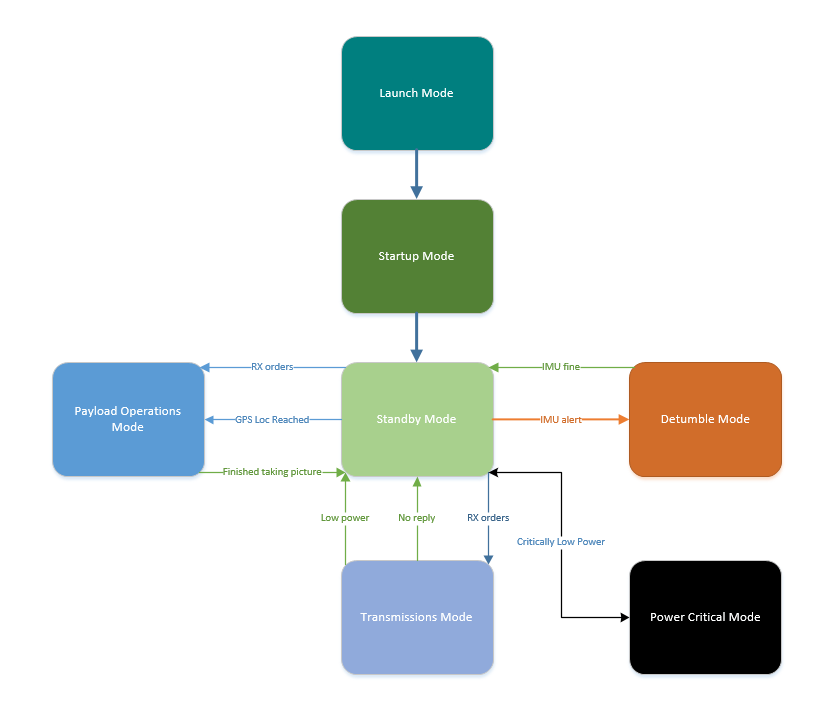
\includegraphics[width=\textwidth]{States.png}
\caption{Mode Transition Diagram during satellite lifetime}
\end{figure}


%%
%%\newpage
%%%\section{Structural Design}
%The proposed one-unit satellite structure will be 3D printed using ABS plastic. This method was chosen in preference of an aluminium chassis primarily because of the ease of access of production. 
%%
%%\newpage
%%\section{System Budgets}
This section detail the power and mass budgets of SnapSat. (overview/description)


\subsection{Mass Budget} 
The mass budget is shown in table~\ref{tab:massbudget}, it is ensured that \textit{SnapSat} meets the requirement of a maximum weight of 1kg. The component masses were used to determine the center of gravity for the satellie, it is desirable to keep this located close to the geometric centre as the attitude control system (magneto-torques) are placed on the outermost surfaces. Centroid averaging across all three axes was used to calculate this as follows
\[
x_{cg} = \cfrac{\Sigma x_i\cdot m_i}{\Sigma m_i} \qquad y_{cg} = \cfrac{\Sigma y_i\cdot m_i}{\Sigma m_i} \qquad z_{cg} = \cfrac{\Sigma z_i\cdot m_i}{\Sigma m_i}
\]
\noindent
The moment of inertia about all three axes is given by
\[ I = \int r^2\,\,dm \]
\noindent
The inertial of each individual component was ignored, assuming these were roughly symmetrical. Only the relative locations of the component contributed to the total inertia. Thus, the inertias were given
\begin{eqnarray} 
I_{xx} &=& \cfrac{1}{\Sigma m_i}\,\cdot\,\left( \Sigma \sqrt{(y_i-y_{cg})^2+(z_i-z_{cg})^2}\,\cdot\,m_i \right) \\
I_{yy} &=& \cfrac{1}{\Sigma m_i}\,\cdot\,\left( \Sigma \sqrt{(x_i-x_{cg})^2+(z_i-z_{cg})^2}\,\cdot\,m_i \right) \\
I_{zz} &=& \cfrac{1}{\Sigma m_i}\,\cdot\,\left( \Sigma \sqrt{(x_i-x_{cg})^2+(y_i-y_{cg})^2}\,\cdot\,m_i \right) 
\end{eqnarray} 
\noindent
and so on; where $x_i$, $y_i$ and $z_i$ are the positions of each component and $m_i$ is the mass of each component. The inertial matrix was computed using \textit{Solidworks}. It was found to be:
\begin{equation}
    I = \bmat{0.4cm}{I_{xx} * I_{xy} * I_{xz} @
                 I_{yx} * I_{yy} * I_{yz} @
                 I_{zx} * I_{zy} * I_{zz}} =
\end{equation}

%\begin{landscape}
\begin{table}[H]
    \centering
    \caption{SnapSat Mass Budget}
    \vspace{0.15cm}
    \label{tab:massbudget}
    {\renewcommand{\arraystretch}{1.3}%
    \begin{tabular}{|>{\arraybackslash}m{3cm}||>{\arraybackslash}m{2.5cm}|>{\arraybackslash}m{2.5cm}|>{\arraybackslash}m{2.3cm}|>{\arraybackslash}m{2.3cm}|}
            \hline
            {\bf Subsystem} & {\bf Mass (g)} & {\bf Contingency (g)} & {\bf Mass and Contingency} & {\bf Fraction of Total Mass} \\ \hline\hline
            Structural &  &  &  &  \\ \hline
            ADCS &  &  &  &  \\ \hline
            EPS &  &  &  & \\ \hline
            OBS / OBDH &  &  &  & \\ \hline
            TT\&C &  &  &  &  \\ \hline
            Thermal &  &  &  &  \\ \hline
            Payload &  &  &  &  \\ \hline
            Integration &  &  &  &  \\ \hline\hline
            Total &  &  &  & \\ \hline
            Mass Margin &  &  &  &  \\ \hline
    \end{tabular} } 
\end{table} \vspace{0.3cm}
%\end{figure} 
%\end{landscape}


\subsection{Power Budget}
\vspace{-0.3cm}
\begin{table}[H]
    \centering
    \caption{SnapSat Power Budget}
    \vspace{0.15cm}
    \label{tab:designoverview}
    {\renewcommand{\arraystretch}{1.4}%
        \begin{tabular}{|>{\arraybackslash}m{2cm}||>{\arraybackslash}m{2cm}|>{\arraybackslash}m{2cm}|>{\arraybackslash}m{1.4cm}|>{\arraybackslash}m{1.4cm}|>{\arraybackslash}m{1.4cm}|>{\arraybackslash}m{1.4cm}|>{\arraybackslash}m{1.4cm}|}
           \hline
           \multicolumn{3}{|l|}{} & \multicolumn{5}{l|}{{\bf Average Duty Cycle by Mode (\%)}} \\ \hline
           {\bf Load} & {\bf Power Consumption (W)} & {\bf Number of Units On} & {\it Safe Mode} & {\it Recovery Mode} & {\it Payload Mode} & {\it Other Mode} &  \\ \hline\hline
           OBC &  &  &  &  &  &  &  \\ \hline
           VHF Rx &  &  &  &  &  &  &  \\ \hline
           S-band Tx &  &  &  &  &  &  &  \\ \hline
           Reaction Wheels &  &  &  &  &  &  &  \\ \hline
           Power Board &  &  &  &  &  &  &  \\ \hline
           Camera &  &  &  &  &  &  &  \\ \hline
           etc. &  &  &  &  &  &  &  \\ \hline
           &  &  &  &  &  &  &  \\ \hline
           &  &  &  &  &  &  &  \\ \hline
           &  &  &  &  &  &  &  \\ \hline\hline
           \multicolumn{3}{|l|}{{\bf Sum Loads (W)}} &  &  &  &  &  \\ \hline
           \multicolumn{3}{|l|}{{\bf Efficiency}} &  &  &  &  &  \\ \hline
           \multicolumn{3}{|l|}{{\bf Power Consumed (W)}} &  &  &  &  &  \\ \hline
           \multicolumn{3}{|l|}{{\bf Power Generated (W)}} &  &  &  &  &  \\ \hline
           \multicolumn{3}{|l|}{{\bf Power Margin}} &  &  &  &  &  \\ \hline
        \end{tabular} } 
    \end{table} \vspace{0.3cm}

\subsection{Pointing Budget}
Since this spacecraft is performing Earth observation, it requires a pointing budget. This refers to the ability to orient the spacecraft towards a target having a specific geographical orientation. Along with the pointing accuracy, the satellite needs to be able to map the location from its own location. Errors in both pointing and mapping accuracies will be discussed here.

\subsection{Link Budgets}
Calculations for both link budgets (list assumptions here).

\subsubsection{Uplink Budget}
The uplink budget allows for XXX. The specifications are
\begin{itemize}
    \item Antenna type at satellite: (omni, directional$+$gain)
    \item Frequency Band: (VHF (145.800MHz) , UHF (435.xxx MHz), SHF etc.)
    \item Objective C/N:
    \item Bit rate and modulation type:
    \item Expected occupied bandwidth:
\end{itemize}

\subsubsection{Downlink Budget}
The downlink budget allows for XXX. The specifications are
\begin{itemize}
    \item Antenna type at satellite: (omni, directional$+$gain)
    \item Frequency Band: (VHF (145.800MHz) , UHF (435.xxx MHz), SHF etc.)
    \item Objective C/N:
    \item Bit rate and modulation type:
    \item Expected occupied bandwidth:
\end{itemize}

\subsection{Data Budget}
Data budget CALCULATIONS.




%%
%%\newpage
\section{Project Plans and Schedule}
A general schedule for the SnapSat project is outlined below. A Gantt chart is provided on the following page.
\begin{table}[H]
    \centering
    \caption{SnapSat Project Schedule}
    \vspace{0.15cm}
    \label{tab:designoverview}
    {\renewcommand{\arraystretch}{1.4}%
        \begin{tabular}{|>{\arraybackslash}m{3.5cm}|>{\arraybackslash}m{4cm}|>{\arraybackslash}m{3.2cm}|>{\arraybackslash}m{3.2cm}|}
            \hline
            \textbf{Major Task} & \textbf{Responsibility} & {\bf Start Date} & {\bf End Date} \\ \hline\hline
             & & & \\\hline
             & & & \\\hline
             & & & \\\hline
             & & & \\\hline
             & & & \\\hline
        \end{tabular} } 
    \end{table}
    
\subsection{Gantt Chart}
\begin{gantt}[xunitlength=0.9cm,drawledgerline=true]{31}{13}
  \begin{ganttitle}
     \numtitle{1}{1}{9}{1}
     \titleelement{-}{1}
     \numtitle{10}{1}{12}{1}
  \end{ganttitle}
        
    \ganttgroup{Preliminary Design\qquad\quad}{0}{4}
    \ganttbar{Component Selection\qquad\quad}{0}{3}
    \ganttbar[color=NavyBlue]{Structural Design\qquad\quad}{1}{3}
    \ganttbar{Link Budgets\qquad\quad}{2}{2}
    \ganttbar{Mass Budgets\qquad\quad}{2}{2}
    \ganttbar{Power Budgets\qquad\quad}{2}{2}
    
    \ganttgroup{Critical Design\qquad\quad}{4}{9}
    \ganttbar[pattern=crosshatch]{Component Reselection\qquad\quad}{3}{2}
    \ganttbar{Budget Reevaluation\qquad\quad}{5}{1}
    \ganttbar{PCB Design and Order\qquad\quad}{4}{3}
    \ganttbar{Thermal Design\qquad\quad}{4}{4}
    \ganttmilestone[color=NavyBlue]{Order Componenets\qquad\quad}{6}
    \ganttbar[color=NavyBlue]{Finalise/Send Structure\qquad\quad}{5.5}{1.5}
    \ganttbar{Report Compilation\qquad\quad}{6}{7}
    
    \ganttgroup{Code Development\qquad\quad}{3}{8}
    \ganttbar{Environment Model\qquad\quad}{3}{3}
    \ganttbar{Simulink Model\qquad\quad}{3}{4}
    \ganttbar{Arduino\qquad\quad}{4}{6}
    \ganttbar{Interface\qquad\quad}{5}{6}
    
    
    \ganttgroup{Componenet Testing\qquad\quad}{9}{3}
    \ganttbar[pattern=crosshatch]{Receive Components\qquad\quad}{9}{2}
    \ganttbar{Thermal System Testing\qquad\quad}{9}{2}
    \ganttbar{ADCS Testing\qquad\quad}{10}{2}
    \ganttbar{Link Testing\qquad\quad}{10}{2}
    \ganttbar{Solar Cell Testing\qquad\quad}{10}{2}
    \ganttbar[color=NavyBlue]{Vibration and Intgeration\qquad\quad}{11}{1}
    
    \ganttgroup{Launch Preparation\qquad\quad}{10}{3}
    \ganttbar[color=NavyBlue,pattern=crosshatch]{Assembly\qquad\quad}{10}{2}
    \ganttbarcon{Final Testing\qquad\quad}{12}{1}
    \ganttmilestonecon[color=red]{Balloon Launch\qquad\quad}{13}
    
%    \ganttcon{11}{21}{10}{28}
\draw[-latex,rounded corners=1.5pt] (5\ganttunitlength,-8+0.1 + 0.2) -- (5\ganttunitlength+0.4*\ganttunitlength,-8+0.1+0.2) -- (5\ganttunitlength+0.4*\ganttunitlength,-8-0.4+0.2) -- (5\ganttunitlength-1.4*\ganttunitlength,-8-0.4+0.2) -- (5\ganttunitlength-1.4*\ganttunitlength,-12+0.1+0.2) -- (6\ganttunitlength,-12+0.1+0.2);

\draw[-latex,rounded corners=1.5pt] (6\ganttunitlength,-12+0.1 + 0.2) -- (6\ganttunitlength+0.4*\ganttunitlength,-12+0.1+0.2) -- (6\ganttunitlength+0.4*\ganttunitlength,-12-0.4+0.2) -- (6\ganttunitlength-3.4*\ganttunitlength,-12-0.4+0.2) -- (6\ganttunitlength-3.4*\ganttunitlength,-21+0.1+0.2) -- (9\ganttunitlength,-21+0.1+0.2);
    
\draw[-latex,rounded corners=1.5pt] (11\ganttunitlength,-21+0.1 + 0.2) -- (11\ganttunitlength+0.4*\ganttunitlength,-21+0.1+0.2) -- (11\ganttunitlength+0.4*\ganttunitlength,-21-0.4+0.2) -- (11\ganttunitlength-2.4*\ganttunitlength,-21-0.4+0.2) -- (11\ganttunitlength-2.4*\ganttunitlength,-28+0.1+0.2) -- (10\ganttunitlength,-28+0.1+0.2);

\end{gantt}

%%\newpage
%%\section{Comments by Independent Reviewer}
One page maximum. (Not quite sure what this is)
%
%\newpage
%\nocite{*}
%\bibliographystyle{ieeetr}
%\bibliography{bib}
%
%\newpage
%\appendix
%\section{Appendix: Supplementary Plots and Data}

\section{Appendix: MATLAB Codes}

\end{document}

%% ITEM TEMPLATES

%TABLES
%\begin{table}[H]
%    \centering
%    \caption{Maximum Expected Values of Angle of Attack Excursion}
%    \vspace{0.2cm}
%    \label{tab:maxturbulencealpha}
%    {\renewcommand{\arraystretch}{1.4}%
%        \begin{tabular}{|>{\centering\arraybackslash}m{2.5cm}|>{\centering\arraybackslash}m{2.5cm}|}
%            \hline
%            Turbulence Component & Maximum ($3\sigma$ value) \\ \hline\hline
%            $u_g$ & 0.0195\deg \\ \hline
%            $w_g$ & 1.3443\deg \\ \hline
%            $q_g$ & 0.3309\deg \\ \hline
%            All & 1.3846\deg \\ \hline
%        \end{tabular} } 
%    \end{table}